\chapter{Some Chapter Name to be changed}

\section{Diffusion Models}
\subsection{Forward Diffusion Process}

\begin{equation}
	\begin{split}
		q(x_t\mid x_{t-1}) & = \mathcal{N}(\sqrt{1-\beta_t} x_{t-1}, \beta_t I) \\
		q(x_t\mid x_{t-1}) & = \mathcal{N}(\sqrt{\alpha_t} x_{t-1}, (1-\alpha_t) I) \\
		q(x_t\mid x_{0}) & = \mathcal{N}(\sqrt{\bar{\alpha}_t} x_{0}, (1 - \bar{\alpha}_t) I) \\
		\bar{\alpha}_t & = \prod_{i=0}^{t} \alpha_t 
	\end{split}
\end{equation}

\begin{figure}[h]
    \centering
    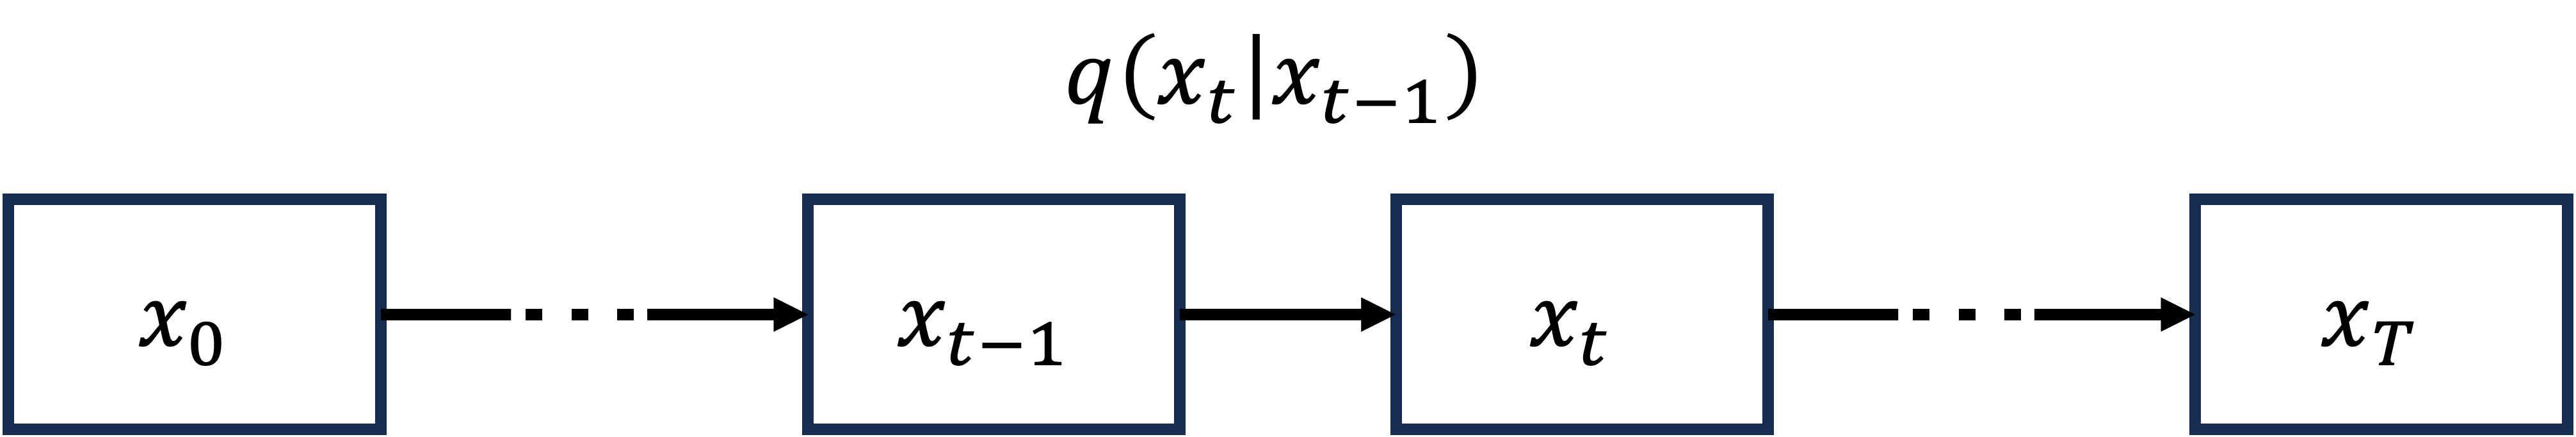
\includegraphics[width=.5\textwidth]{img/forward_diffusion.png}
    \caption{Forward Diffusion Process: An image is iteratively destroyed by adding normally distributed noise, 
    according to a schedule. This represents a Markov process where the transition probability $q(x_t|x_{t-1})$.}
    \label{fig:forward_diffusion}
\end{figure}

\begin{figure}
    \centering
    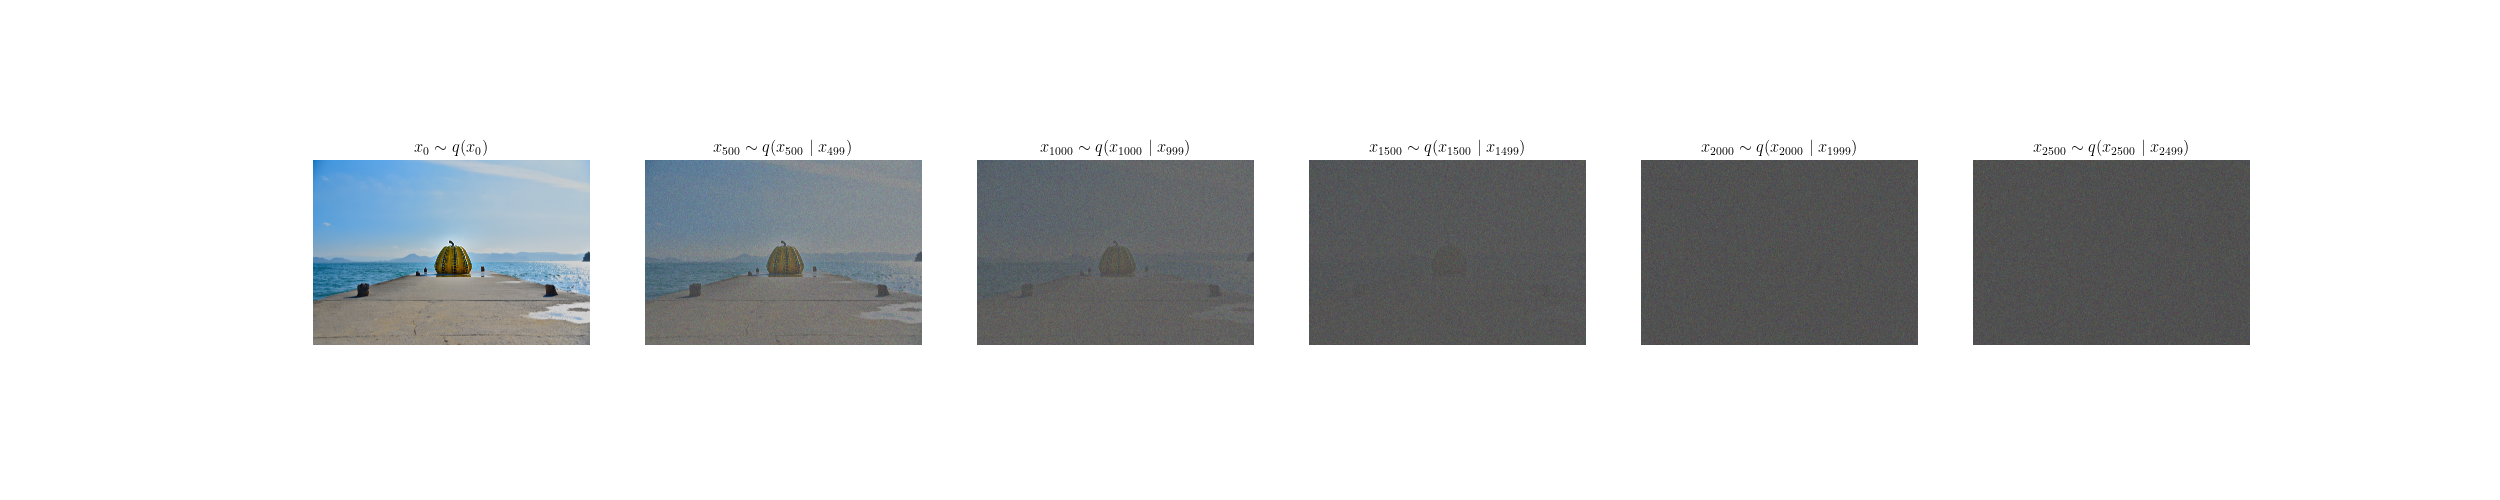
\includegraphics[width=\textwidth]{img/forward_naoshima.png}
    \caption{Example of Iterative Image Destruction through Forward Diffusion Process:
    The indices give the time step in the iterative destruction process, where $\beta$ was created according to a linear noise variance schedule (5000 steps from in the 0.001 to 0.02 range and picture resolution of 4016 by 6016 pixels).}
\end{figure}